% !TEX encoding = UTF-8 Unicode
\documentclass[12pt,a4paper,english
% ,twoside,openright
]{tunithesis}

\special{papersize=210mm,297mm}

\author{Roosa Kuusivaara \& Väinö-Waltteri Granat}
\title{Digital Image Formation And Processing - Report} % primary title (for front page)
\thesistype{Laboratory Report} % or Bachelor of Science, Laboratory Report...

\usepackage{lastpage}
\usepackage[english]{babel}
\usepackage[
backend=biber,
style=authoryear,
citestyle=authoryear,
autocite=inline
]{biblatex}
\usepackage{csquotes}
\usepackage{matlab-prettifier}
\usepackage{svg}

\addbibresource{references.bib} %Imports bibliography file


\definecolor{tunipurple}{RGB}{78, 0, 142}

\newcommand\todo[1]{{\color{red}!!!TODO: #1}} % Remark text in braces appears in red
\newcommand{\angs}{\textsl{\AA}}              % , e.g. slanted symbol for Ångstöm
% Preparatory content ends here


\pagenumbering{roman} % was: {Roman}
\pagestyle{headings}
\begin{document}

% Special trick so that internal macros (denoted with @ in their name)
% can be used outside the cls file (e.g. \@author)
\makeatletter

% Create the title page.
% First the logo. Check its language.
\thispagestyle{empty}
\vspace*{-.5cm}\noindent

\begin{figure}
    \vspace{-1.3cm}
    \advance\leftskip-2.5cm
    \noindent\includegraphics{img/tunilogo.png}
\end{figure}
 
\vspace{2.5cm}
\begin{flushright}
\noindent\textsf{\LARGE{\@author}}

\noindent\vspace{0.5cm}

\noindent\Huge{\textsf{\textbf{\textcolor{tunipurple}{\@title}}}}
\end{flushright}
\vspace{13.7cm} % adjust to 12.7 this if thesis title needs two lines

% Last some additional info to the bottom-right corner
\begin{flushright}  
    \begin{spacing}{1.0}
      \textsf{Faculty of Information Technology and Communication Sciences (ITC)\\
      \@thesistype\\}
    \end{spacing}
\end{flushright}

% Leave the backside of title page empty in twoside mode
\if@twoside
\clearpage
\fi

% Turn off page numbering for the first pages
\pagenumbering{gobble}


% Some fields in abstract are automated, namely those with \@ (author,
% title, thesis type).
\chapter*{Abstract}
\begin{spacing}{1.0}
\noindent \@author: \@title\\
\@thesistype\\
Tampere University\\
Master’s Degree Programme in Signal Processing\\
December 2023
\end{spacing}
\noindent\rule{12cm}{0.4pt}

\vspace{0.5cm}

% ---------------------------------------
% Abstract and keywords
% ---------------------------------------

\noindent
This report documents the work done in the Digital Image Formation And Processing assignment as a part of the Advanced signal processing laboratory course. In this assignment we familiarized ourselves with basics of digital image formation from raw sensor data as well as image processing.

~

\noindent\textbf{Keywords:} Image processing, Image formation.

~

\noindent The originality of this thesis has been checked using the Turnitin Originality Check service.


% Add the table of contents


\setcounter{tocdepth}{3}              % How many header level are included
\tableofcontents                      % Create TOC


% The actual text begins here and page numbering changes to 1,2...
% Leave the backside of title empty in twoside mode
\if@twoside
%\newpage
\cleardoublepage
\fi


\renewcommand{\chaptername}{} % This disables the prefix 'Chapter' or
                              % 'Luku' in page headers (in 'twoside'
                              % mode)


\chapter{Introduction}
\label{ch:intro} 
In this report we describe our work done in the 'Digital Image Formation and Processing' laboratory assignment for the Advanced Signal Processing Laboratory course. In this assignment we implemented a basic raw image formation and processing pipeline in Matlab to construcut RGB images from raw sensor data.

\pagenumbering{arabic}
\setcounter{page}{1} 

\chapter{Methodology}
\label{sec:methodology}
In this section we will present our implementation of the image processing pipeline, by going over the main parts of the Matlab code as well as explaining the the decisions we took when requirements we ambigious.

\section{Overview of the pipeline}
Figure~\ref{fig:pipeline} shows the complete image processing and formation pipeline that we are going to introduce in this report. The following sections will go over the different parts of the pipeline. The pipeline takes in raw sensor data of Bayer arrays in RGGB format and produces RGB images. In addition to image formation the pipeline also performs focusing, white balancing and contrast and saturation correction.

\begin{figure}
  \centering
  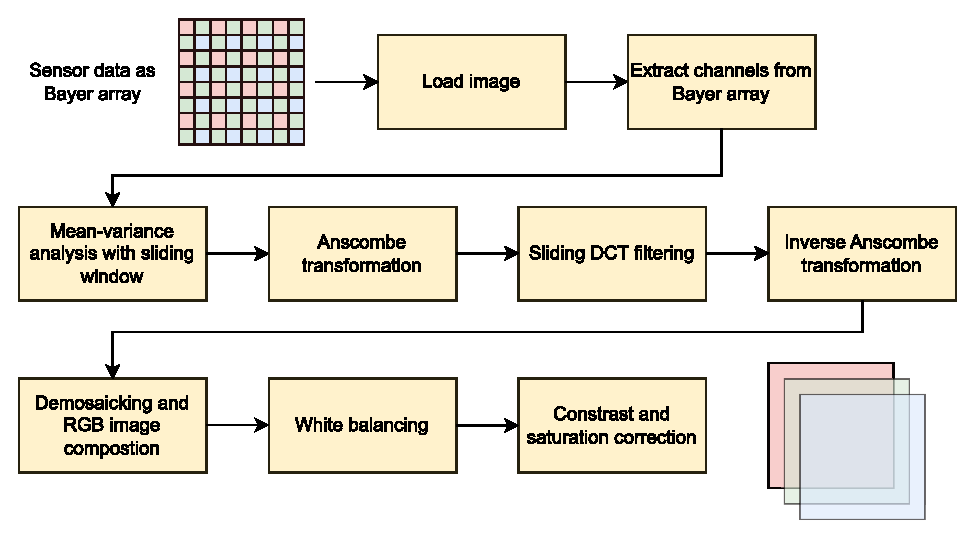
\includegraphics[width=0.8\textwidth]{img/image_pipeline.eps}
  \caption{Our image processing and formation pipeline}
  \label{fig:pipeline}
\end{figure}

\section{Reading images and converting to doubles}

\section{Image visualization and Bayer mosaic}

\section{Sliding window}

\section{Scatterplots and regression}

\section{Transformation and reverse transformation}

\section{DCT denoising}
\begin{lstlisting}[style=Matlab-editor, numbers=left, basicstyle=\small]
function [denoised] = DCTImageDenoising(image, lambda, transformBlockSize)

    % Create a custom function to be applied to each block
    fun = @(block_struct) idct2(thresholdDCT(block_struct.data, lambda));

    % Apply the function to each block
    denoised = blockproc(image, transformBlockSize, fun);
end

function denoised = thresholdDCT(input, lambda)

    % Apply DCT to the block
    dctBlock = dct2(input);

    % Threshold the DCT coefficients
    dctBlock(abs(dctBlock) < lambda) = 0;
    denoised = dctBlock;
end
\end{lstlisting}

\section{Demosaicking}

\section{White balancing}

\section{Contrast and saturation correction}



\chapter{Results}
\label{sec:results}
In this section we will present the results from our image processing pipeline and also do some analysis on why we got the kinds of results that we did.

\chapter{Conclusions}
\label{ch:conclusions}

%
% The bibliography, i.e the list of references
%
\newpage

\printbibliography[title=References]
\addcontentsline{toc}{chapter}{References}

\end{document}

